\chapter{Memory formation in Alzheimer's Disease}
\section{Introduction}

\section{Material and Methods}\todo{edit methods}

\subsection{Animals and vectors}
All animals were housed in groups of 4 or 5, with a 12-hour light/dark cycle. Food and water are provided \textit{ad libitum} to all animals. Experiments were performed during the light phase of the circadian cycle. Mice were at least 8 weeks old at the beginning of all experiments. All experiments were in accordance to the Hospital for Sick Children Animal Care and Use Committee.

\subsubsection{TgCRND8 mice}
TgCRND8 mice were developed at the Center of Research for Neurodegenerative Diseases (CRND) and carry a human APP695 transgene with the Swedish (K670N-M671L) and Indiana (V717F) FAD mutations under the regulation of the Syrian hamster prion promoter \citep{chishti01}. TgCRND8 was back-crossed with C57BL/6, \gls{tg} and \gls{wt} littermates of F1 generation were used in the experiments.


\subsubsection{GP5.17 mice}
GP5.17 mice transgenically express the flourescence calcium indicator GCaMP6f under the Thy1 promoter \citep{dana14}. TgCRND8 was crossed with GP5.17. Animals that that are GCaMP6f\textsuperscript{+} and \gls{app}\textsuperscript{-}, or GCaMP6f\textsuperscript{+} and \gls{app}\textsuperscript{+} are used in the experiments. 

\subsubsection{Viral vectors}
In the TgCRND8 mice, GCaMP6f expression is delivered through \gls{aav}. GCaMP6f expression is controlled by \gls{hsyn} promoter. AAV--DJ--syn--GCaMP6f virus was purchased from Stanford University Gene and Viral Vector Core. The virus is used undiluted. 

\subsubsection{\tglu~peptide}
To deliever \glu~construct (YKEGYNVYG) to target, we attached it to the protein transduction domain of the \gls{hiv} \textit{tat} gene (TAT peptide). The TAT peptide is able to transport across cell membrane and \gls{bbb} through an unknown mechanism \todo{cite TAT}. The \tglu was synthesized from the sequence YGRKKRRQRRRYKEGYNVYG and desolved in saline. 


\subsection{Viral Infusion}

Each animal received \gls{ip} injection of atropine (\SI{0.1}{\mg\per\kg}) and chlorohydrate (\SI{400}{\mg\per\kg}) before being secured on a stereotaxic frame. An incision was made on the scalp and the skin was pulled to the side to reveal the skull. Holes were drilled above \gls{la} on the skull for micropipette injection. Virus was loaded into a glass micropipette and gradually lowered to target coordinate. \SI{1.5}{\ul} of virus were injected on each side at a rate of \SI{0.12}{\ul\per\min}, aiming at \gls{la} (\gls{a/p} \SI{-1.4}{\mm}, \gls{m/l} $\pm$\SI{3.5}{\mm}, \gls{d/v} \SI{5.0}{\mm} from Bregma). The micropipette was left in the brain for an extra \SI{10}{\min} before slowly retracted. The incision was sutured and treated with antibiotics. Each animal then received subcutaneous injection of analgesic (ketoprofen, \SI{5}{\mg\per\kg}) before returned to a partially heated clean cage for recovery.

\subsection{Histology}
Placement of implants and extent of viral infections was determined by \gls{gfp} expression. After all experiments, animals were transcardially perfused with first \gls{pbs} then 4\% \gls{pfa}. The brains were disected and kept in 4\% \gls{pfa} overnight, and washed with \gls{pbs}. The brains were then sliced coronally on a vibrotome (\todo{vibrotome info}) to \SI{50}{\um} thickness. Slices containing \gls{la} were then mounted on gelatin-coated glass slices with a hardening mounting media (Permaflour\todo{permaflour info}) and assessed under an epi-flourescence microscope(Nikon\todo{Nikon info}).

\subsection{Contextual fear conditioning}
Fear conditioning chambers (\SI{31 x 24 x 21}{\cm}; MED Associates, St. Albans, VT), consisted of 2 stainless steel and 2 clear acrylic walls, with a stainless steel shock-grid floor (bars \SI{3.2}{\mm} diameter, spaced \SI{7.9}{\mm} apart). A plastic drop-pan containing a 70\% ethanol solution was placed below the grid floor. A fan provided low-level white- noise during training and testing in the context. Behavior was monitored by overhead cameras, which digitized video images at \SI{15}{\Hz}. 

Animals underwent contextual fear conditioning three weeks after mini-microscope baseplate implantation. One hour before training, animals received either TAT-GluA2 peptide (i.p., \SI{15}{\mmol\per\kg}) or vehicle injection. A mini-microscope is attached to the animal to record calcium activities during both training and testing of contextual fear conditioning. During training, animals were confined in the chamber for \SI{5}{\minute}. A footshock of \SI{0.5}{\mA} was delivered at \SI{4}{\minute} time point. During testing session \SI{24}{\hour} later, animals were placed back in the training environment for \SI{10}{\minute}. 

\subsection{Animal tracing}
\todo{Animal tracing method}
Videos of animal behaviours were encoded as grey-scale images. Due to a dark background, overlaying mini-microscope wire and commutators and changing shadows, no simple feature is able to reliably identify the animal from the background. Instead, we used multiple features, calculate the distribution of the features in tracked animals, and use all the features together to estimate the position of the animal for each frame.

\subsubsection{Features}

A background image of the environment was generated by taking the mean pixel density across time. 

\begin{table}
    \begin{tabular}{|c|c|p{3cm}|}
        \hline
        \textbf{Feature Name} & \textbf{Formula} & \textbf{Description} \\ \hline
        Pixel intensity & $p_i^t$ & Intensity of pixel \\ \hline
        Normed pixel intensity & $\displaystyle \frac{p_i^t - E(p^t)}{\sigma(p^t)}$ & Pixel intensity when frame is normalized to zero mean and unit standard deviation \\ \hline
        Foreground pixel intensity & $p_i^t - p_i^{bg} $ & Intensity difference between pixel and background pixel \\ \hline
        Difference to low pass intensity & $p_i^t - (lp(p^t))_i$ & \\ \hline
        Speed & $dist(p_i^t, p^{t-1})$ & distance to animal position in the last frame \\ \hline
        change in intensity & $p_i^t - p^{t-1}$ & Difference to pixel intensity at the animal position in the last frame \\ \hline
        change in intensity (blurred) & $blur(p^t)_i - blur(p^{t-1})_i$& Difference to pixel intensity at the animal position in the last frame blurred \\ \hline
        Acceleration &$ |velocity(p^t) - velocity(p^{t-1})|$& Difference of speed to last frame \\ \hline
        Area & $s$ & Area of the pixel in when the frame is edge detected and morphologically closed \\ \hline
    \end{tabular}
\end{table}

\subsubsection{Training}
During training, the value of every feature was calculated at the pixel of the ground truth position of the animal. A probability distribution was estimated, and stored. 

\subsubsection{Tracking}
\todo{particle filter}
The tracking is done in a frame-to-frame basis. For a single pixel, we calculate its score as the summation of likelihood for all the features\todo{formula}. The pixel with the highest score is the most likely position of the animal. However, calculating score for every pixel is computationally intensive. Instead, we took advantage of particle filters to estimate the distribution of score over pixels. \todo{cite particle filters, formula, detailed description}.

While improvement can still be made to this method, with the current implementation the algorithm is able to correctly track animals with minimal human intervention. \todo{ref code}


\subsection{Analysis}

All traces were normalized to have zero median and unit noise standard deviation. The noise standard deviation was estimated from median absolute deviation of the trace. The signal to noise ratio (SNR) were calculated as the ratio of maximum signal intensity and noise standard deviation. Only traces with more than 10 SNR and animals with more than 20 cells are included in the analysis. The average activity of a cell was calculated by the area under the calcium trace above 3 standard deviation of the noise divided by duration.

Freezing information and spatial information (below) were calculated according to \citet{skaggs93}. The information measurement represents how much cell activity at a single time can predict about freezing or location of the animal.  It was calculated using the following formula:

$Information = \displaystyle\sum_{i}^{}P_i  \frac{R_i}{R} log_2 \frac{R_i}{R}$

where $P_i$ represents the probability of the animal being in state $i$,  $R_i$ represents the average cell activity when the animal is in state $i$, and $R$ is the average cell activity during the session. For freezing, the states are freezing and not freezing. For spatial information, environment is divided in \num{12 x 9} grids, and the states are when animal is in one of the grids.

\section{Results}
First, we compared the average activity between groups, and have found the Tg animals are hyper-active. We have then investigated the average cell activity during freezing, and found CA1 cells decrease activity to encode freezing. However, Tg animals have higher activity during freezing than WT animals. This suggest Tg animals may have 

We then investigated that how cell Tg cells encodes freezing. First we looked at cells individually, and calculated the mutual information between cell firing and freezing (Skaggs et al., 1993). Then using machine learning methods, we investigated how freezing is encoded at a network level by training general classifiers to predict animals' behaviour from recorded cell activity. Both approach suggest that Tg animals have consistent worse freezing encoding both at a cellular level but also at a network level. 

We have also investigated how the animals freeze, by A detailed analysis of the animals' freezing behaviour suggests that the Tg animals often start to freeze, however each freezing period is significantly 


The experimental paradigm is summarized in Figure~\ref{paradigm}. Mini-microscope baseplates were surgically implanted in CA1 hippocampus in gCaMP6f expressing wildtype (WT) and APP transgenic (Tg) animals. To transiently increase surface GluA2 density, we used a short interference peptide (TAT-GluA2\textsubscript{3Y}) to block GluA2-containing AMPAR endocytosis. The animals received either vehicle (Veh) or TAT-GluA2\textsubscript{3Y} (Glu) peptide one hour before training. Twenty-four hours later, the animals were tested in the training chamber. Calcium transients were recorded during both training and testing session of contextual fear conditioning. Figure~\ref{trace} shows cells recorded from a single animal and a sample of calcium traces. 


Figure~\ref{activity} shows overall cell activity during training and testing. Consistent with previous reports in the literature \citep{verret12}, cells in Tg animals have increase overall cell activity. Interestingly, the TAT-GluA2\textsubscript{3Y} administered before the training session corrected the cell activity in Tg to WT levels both during training and during testing. This suggests that either the rescuing effect is long-lasting, or successfully forming and recalling a memory corrects the cell activity to base level.

Figure~\ref{freezing} shows the percent of freezing during testing. Consistent with our hypothesis, Tg animals showed decreased freezing, and this was rescued by TAT-GluA2\textsubscript{3Y} treatment. 

We have further calculated freezing information content. This measurement reflects how much prediction power a cell has for freezing in a period of time. Again, cells in Tg animals have less freezing information, and this effect is partially rescued by TAT-GluA2\textsubscript{3Y} treatment (Figure~\ref{freeze_info}). This result suggests that, not only do the Tg animals freeze less, but when they are freezing, the information is not well encoded in hippocampus CA1. 

However, given that the Tg animals also show behavioural difference, we then try to answer the question: is the difference in neural coding inherit of the Alzheimer animal, or a result of the different behaviour? Given that CA1 cells are known to represent place, we have calculated the freezing information marginalized over all animal positions, therefore eliminating it's effect in the calculation of freezing information. The result is similar and shown in Figure~\ref{freeze_ctrl}. 

In addition, we also checked whether the freezing information coding is a result of different freezing or uneven spatial coverage of the behavioural chamber, which are represented by freezing entropy and spatial entropy respectively. To check these two factors, we have pooled the groups with similar behaviour (WT, WT-GluA2\textsubscript{3Y}, Tg-GluA2\textsubscript{3Y}), and correlated percent freezing, freezing entropy, total distance and spatial entropy against freezing information within the pooled groups. If the behavioural measurement have no influence in the freezing information, we would expect no correlation. Indeed, that is what we have found in Figure~\ref{corrs}. These control measurements have shown that the reduction of freezing encoding in the Tg animals is not affected by the difference in the animals' behaviour.

The next question we investigated is, if the cells are encoding freezing, how do they encode? In figure~\ref{ch_activity} we selected all the cells that have more than 0.01 bits/second (which amounts to ~40\% in the normal groups and 10\% of the cells in the Tg group), and plotted the difference of average activity when the animal is freezing and not freezing. Interestingly, most of the cells encode freezing by decreasing their activity. This can also be seen representatively in the sample trace (Figure~\ref{sample_trace}).

Given the cells tend to have decreased activity during freezing, we also examined the average cell activity when the animal is freezing, and activity when the animal is not (Figure~\ref{activity_freezing}). Consistent with the freezing information result, the Tg animals have higher activity when the animal is freezing, and this is rescued by the TAT-GluA2\textsubscript{3Y}. Interestingly, the rescue group also shows significantly decreased activity when the animal is not freezing. These results suggest the TAT-GluA2\textsubscript{3Y} may rescue the Tg phenotype by globally decrease background cell activity.


While all the measurements we have performed considers each cell individually, are the cells independent of each other, or is part of the information encoded in the coordination between them? To answer this question, we have build two classifiers: a naive bayes (NB) classifier which models the cells independent of each other, and a gaussian support vector machine (SVM), which also uses the dependency between cells for prediction. The result is shown in Figure~\ref{classifier}. The SVM significantly outperforms the NB classifier, suggesting that the network encodes more information than the cells individually. Moreover, both classifiers perform significantly worse in the Tg group, further supports our hypothesis that Tg animals have inferior fear memory encoding.

\subsection{Freezing Behaviour}
\todo{paradigm}
\begin{figure}[h]
    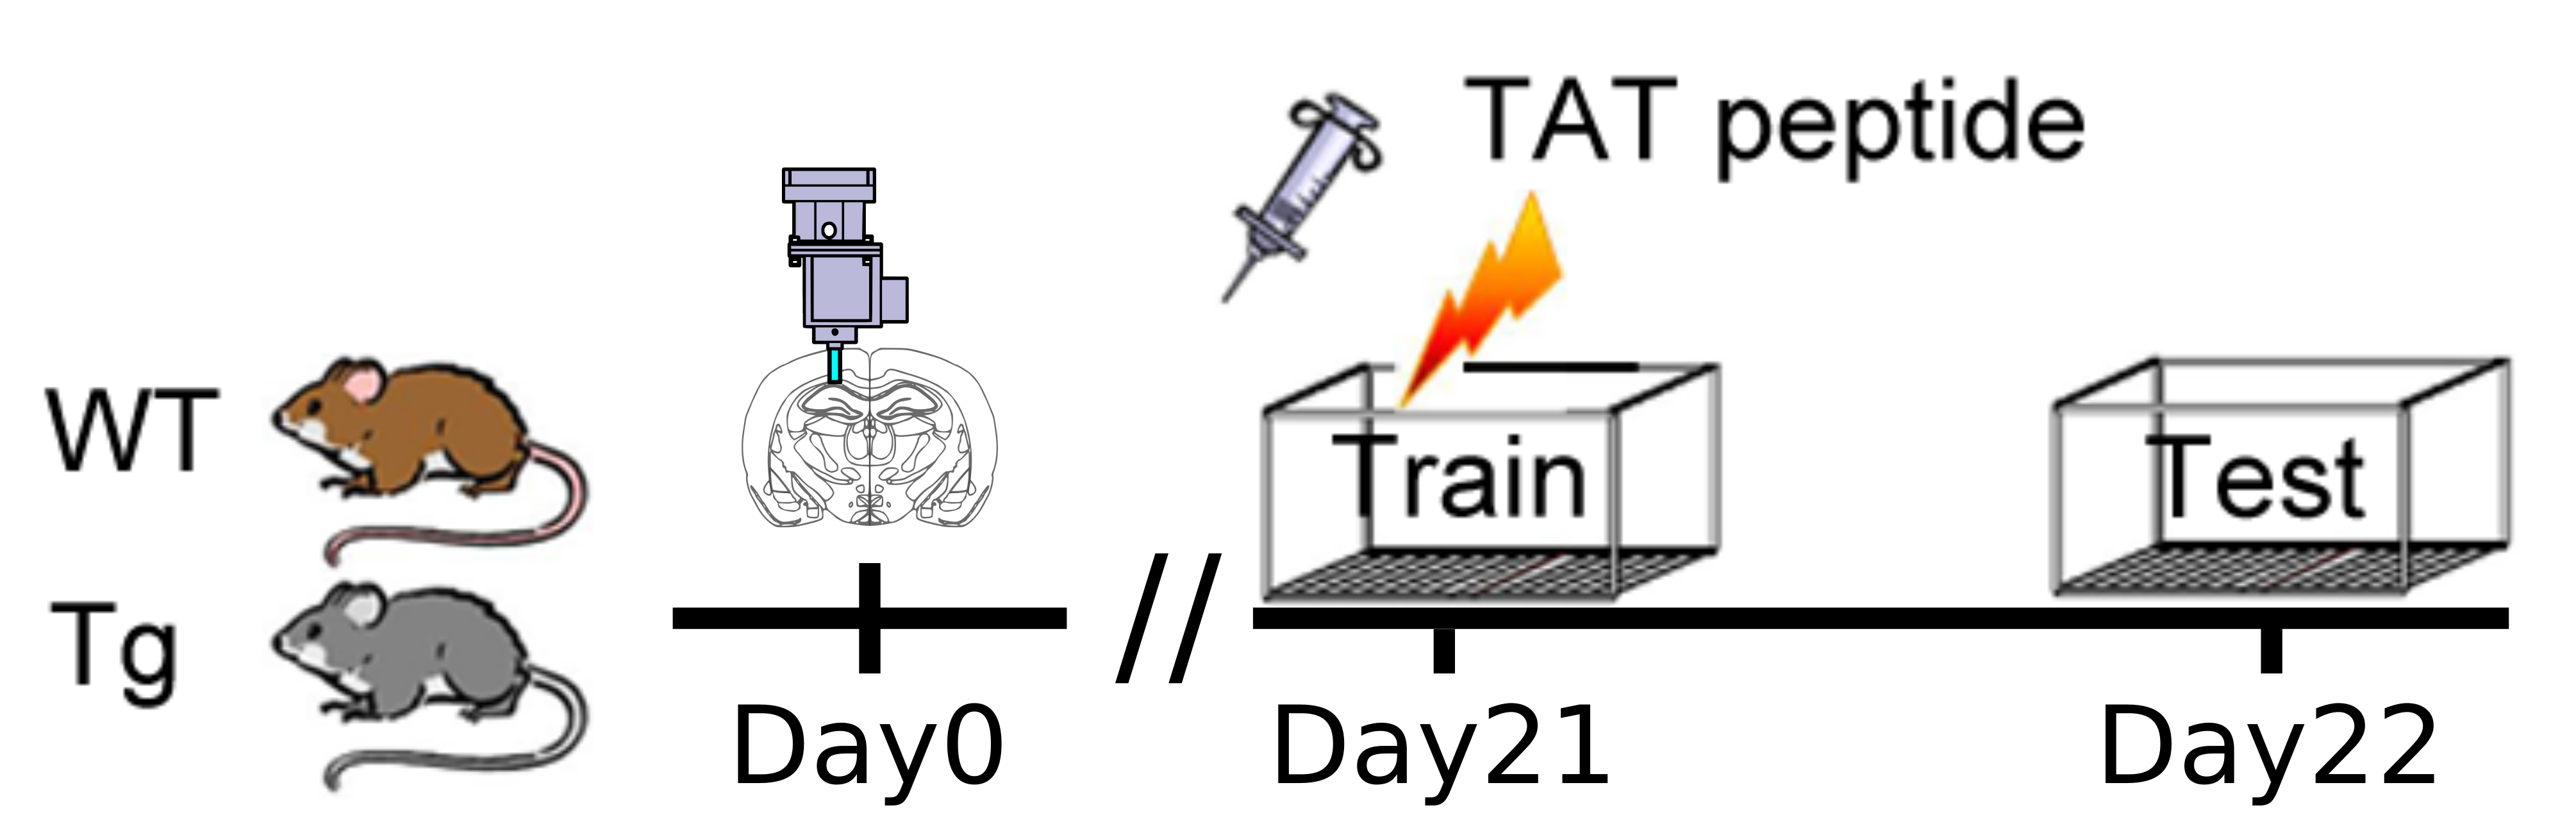
\includegraphics[width=\textwidth]{paradigm.png}
    \caption{Experimental paradigm. Adult \gls{wt} and \gls{tg} animals (with gCaMP6f expression) were implanted with a mini-microscope baseplate targeting CA1 hippocampus on day 0. The cells were visible three weeks later. Animals received \tglu peptide (i.p.) \SI{1}{\hour} before contextual fear conditioning. Animals were tested \SI{24}{\hour} later for freezing behaviour. Calcium activity were recorded for both training and testing session. \label{f.ad.paradigm}}
\end{figure}

\begin{figure}[h]
    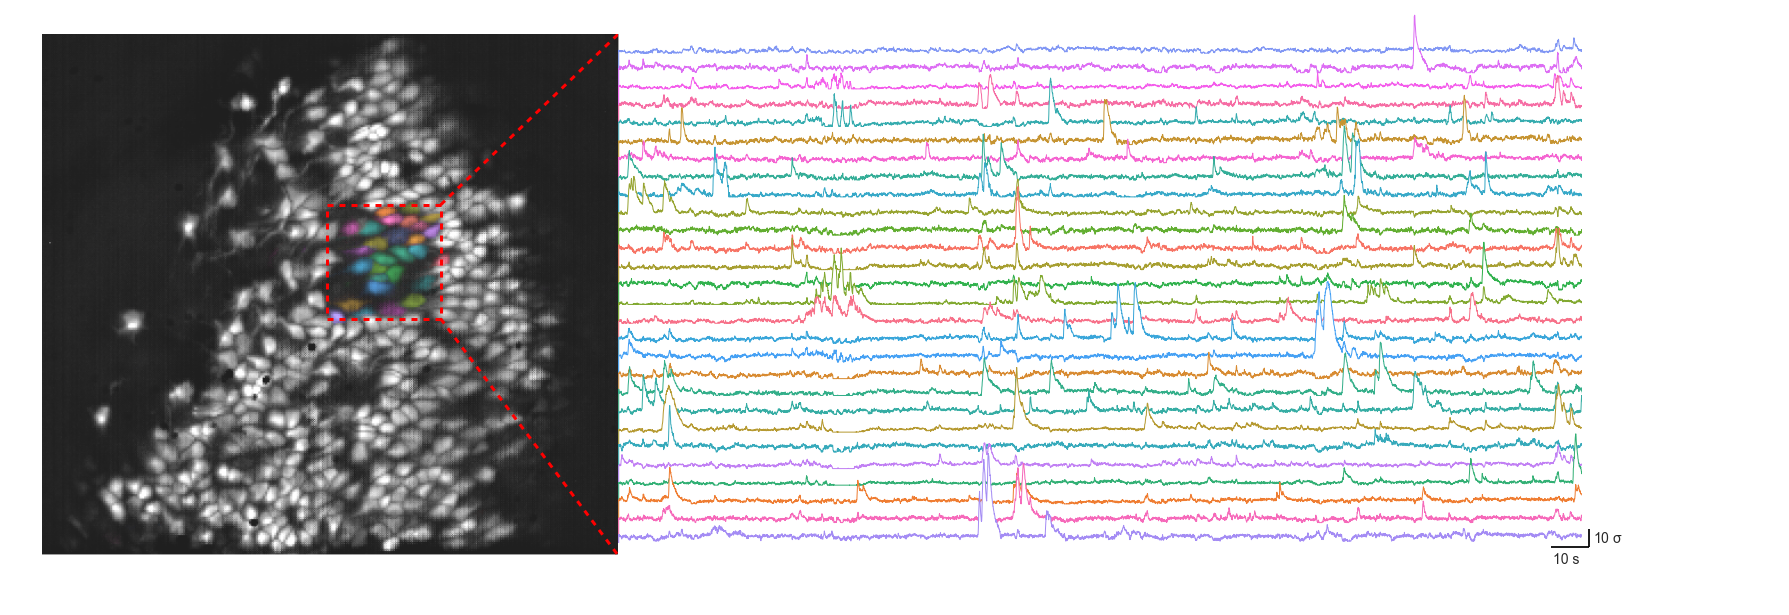
\includegraphics[width=\textwidth]{trace.png}
    \caption{Sample cell image and traces. Traces are random coloured and correspond to cells of the same colour. \label{f.ad.trace}}
\end{figure}


\todo{freezing}
\begin{figure}[h]
    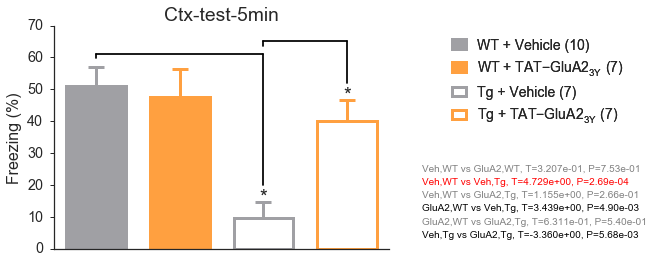
\includegraphics[width=\textwidth]{freezing.png}
    \caption{Percent of freezing during testing. \Gls{tg} animals showed significant lower freezing, and \tglu treatment returns the freezing to wildtype level. \label{f.ad.freezing}}
\end{figure}

\subsection{\tglu rescues hyperactivity in \gls{tg} cells}
\begin{figure}[h]
    \begin{subfigure}[h]{\textwidth}
        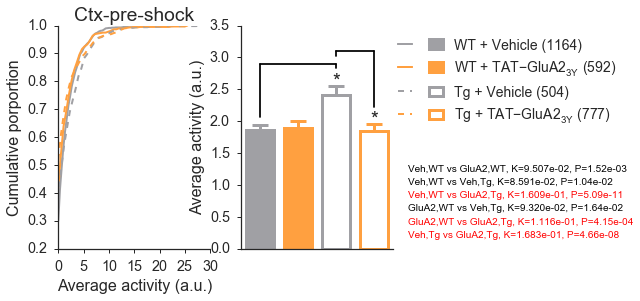
\includegraphics[width=\textwidth]{activity_train.png}
        \caption{\label{f.ad.acttrain}}
    \end{subfigure}
    \begin{subfigure}[h]{\textwidth}
        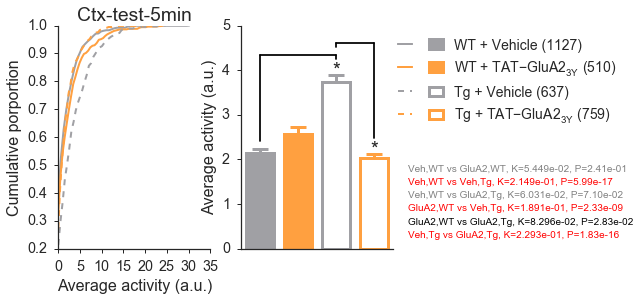
\includegraphics[width=\textwidth]{activity_test.png}
        \caption{\label{f.ad.acttest}}
    \end{subfigure}
    \caption{Distribution and mean of average cell activity during \subref{f.ad.acttrain} training and \subref{f.ad.acttest} testing. Cells in the Tg animals are significantly more active, and this is rescued by \tglu treatment. \label{f.ad.activity}}
\end{figure}

\subsection{\tglu rescues freezing encoding deficit in \gls{tg} cells}
\begin{figure}[h]
    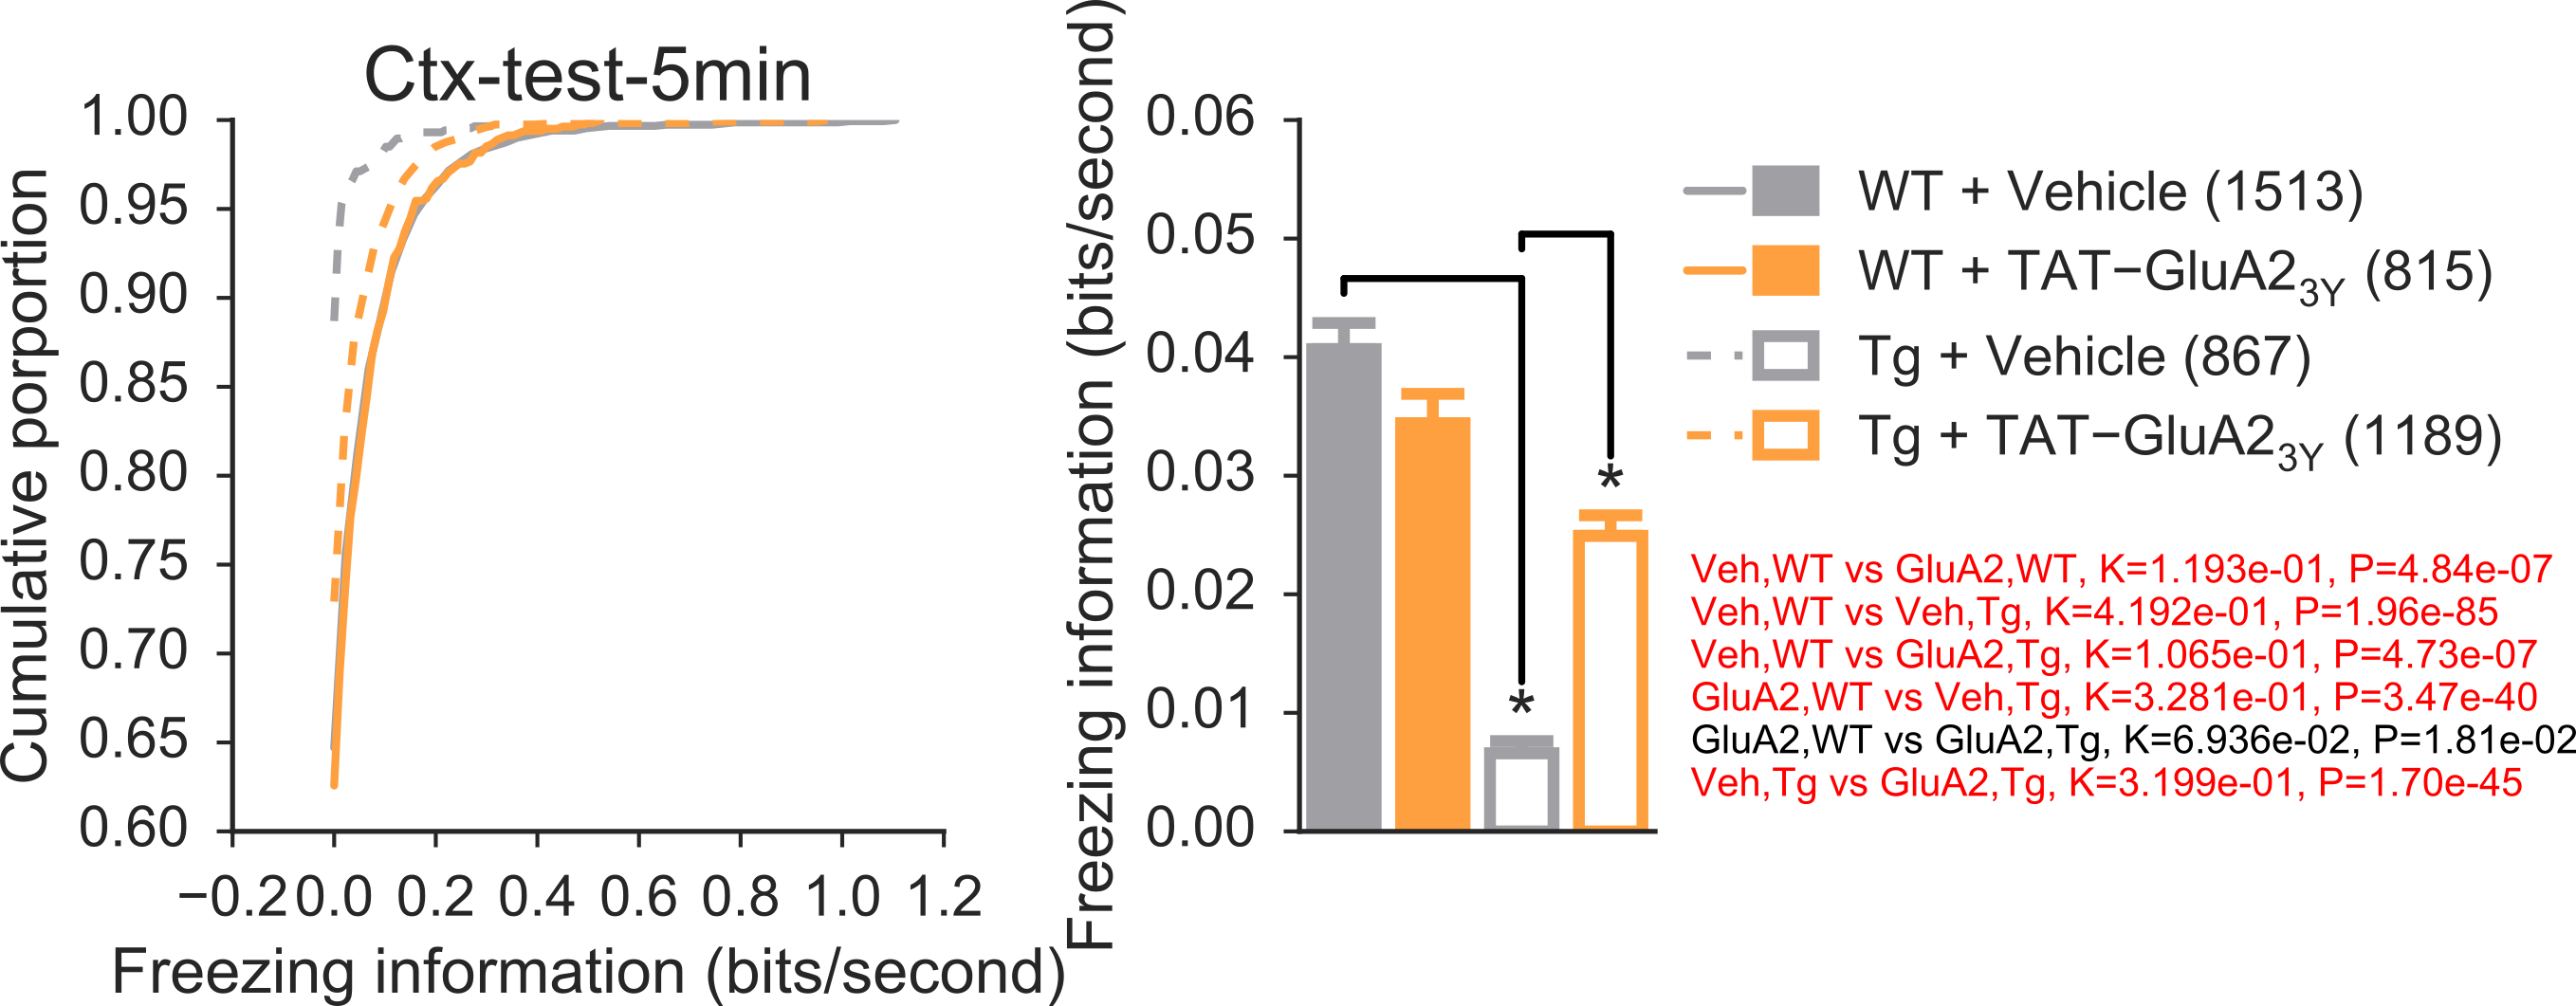
\includegraphics[width=\textwidth]{freeze_info.png}
    \caption{Freezing information during testing. This measurement represent how much information a cell have in a period of time about whether the animal is freezing. Cells in \gls{tg} animals encode significantly less freezing than the \gls{wt} groups, and \tglu treatment can only partially rescue the effect. \label{f.ad.freeze_info}}
\end{figure}
    

\begin{figure}[h]
    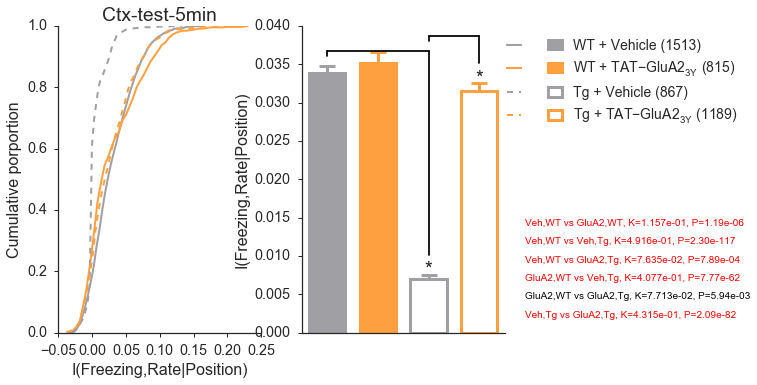
\includegraphics[width=\textwidth]{freeze_position.png}
    \caption{Freezing information conditioned on animal's position. This measurement removes the effect of position from freezing information measurement, and the result is similar to Figure~\ref{f.ad.freeze_info}. This suggest that the position of the animal is not a confounding factor for freezing information measurement. \label{f.ad.freeze_ctrl}}
\end{figure}

\begin{figure}[h]
    \begin{subfigure}[h]{\textwidth}
        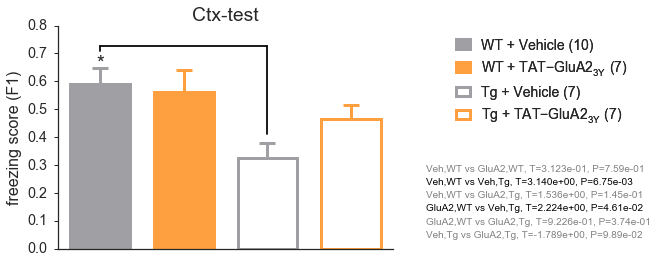
\includegraphics[width=\textwidth]{nb.png}
        \caption{\label{f.ad.nb}}
    \end{subfigure}
    \begin{subfigure}[h]{\textwidth}
        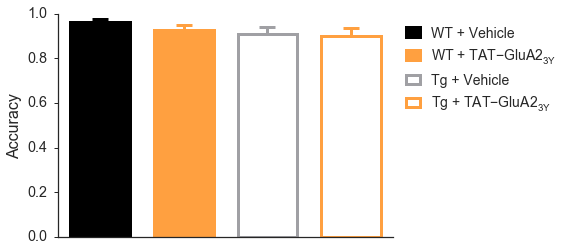
\includegraphics[width=\textwidth]{svm.png}
        \caption{\label{f.ad.svm}}
    \end{subfigure}
    \caption{Performance of \subref{f.ad.nb} \gls{nbc} and \subref{f.ad.svm} \gls{gsvm} in predicting freezing from cell activity. Results are measured as F1 score. Both classifiers showed inferior performance in \gls{tg} group, further supports the hypothesis that \gls{tg} animals have sub-optimal freezing encoding. Interestingly, since \gls{nbc} assumes the cells are independent and \gls{gsvm} is more general, the performance difference between the two suggest a portion of freezing information is encoded in the coordination between the activity of the cells. \label{f.ad.classifier}}
\end{figure}


\subsection{\Gls{tg} animals can initiate freezing}
\subsection{\Gls{tg} animals have deficits recall freezing memory}
\subsection{\tglu rescues recall by decreasing activity}

\begin{figure}[h]
    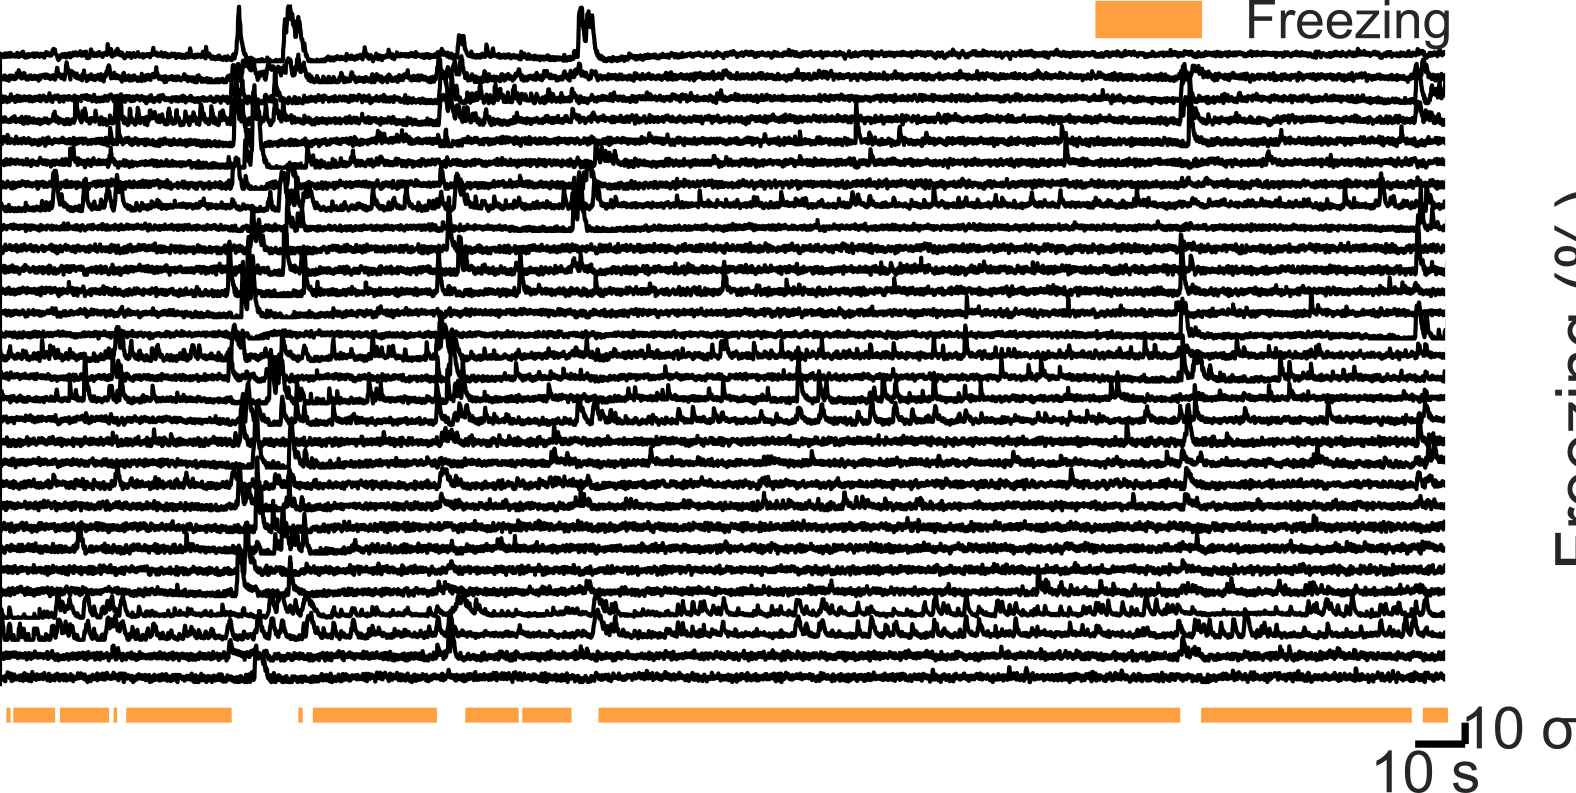
\includegraphics[width=\textwidth]{sample_trace.png}
    \caption{Sample traces from cells with highest freezing information in an animal. It appears that cells encode freezing by decreasing their activity. \label{f.ad.sample_trace}}
\end{figure}

\begin{figure}[h]
    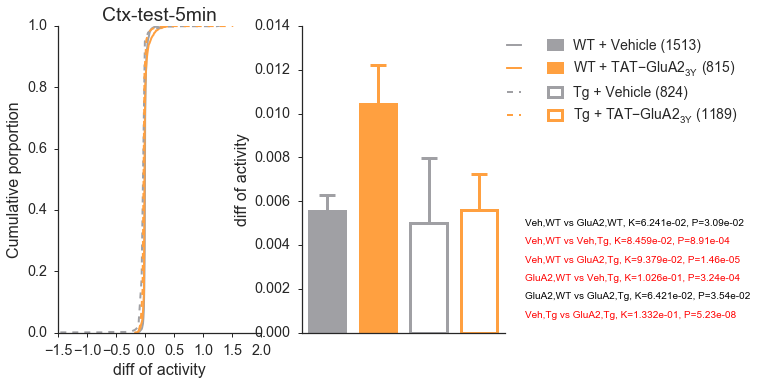
\includegraphics[width=\textwidth]{ch_activity.png}
    \caption{Distribution and mean of activity difference between freezing and none-freezing, in cell with freezing information more than 0.01. This confirms the intuition from Figure~\ref{f.ad.sample_trace} that most of the cells encode freezing by decreasing activity. \label{f.ad.ch_activity}}
\end{figure}





\begin{figure}[h]
    \begin{subfigure}[t]{.5\textwidth}
        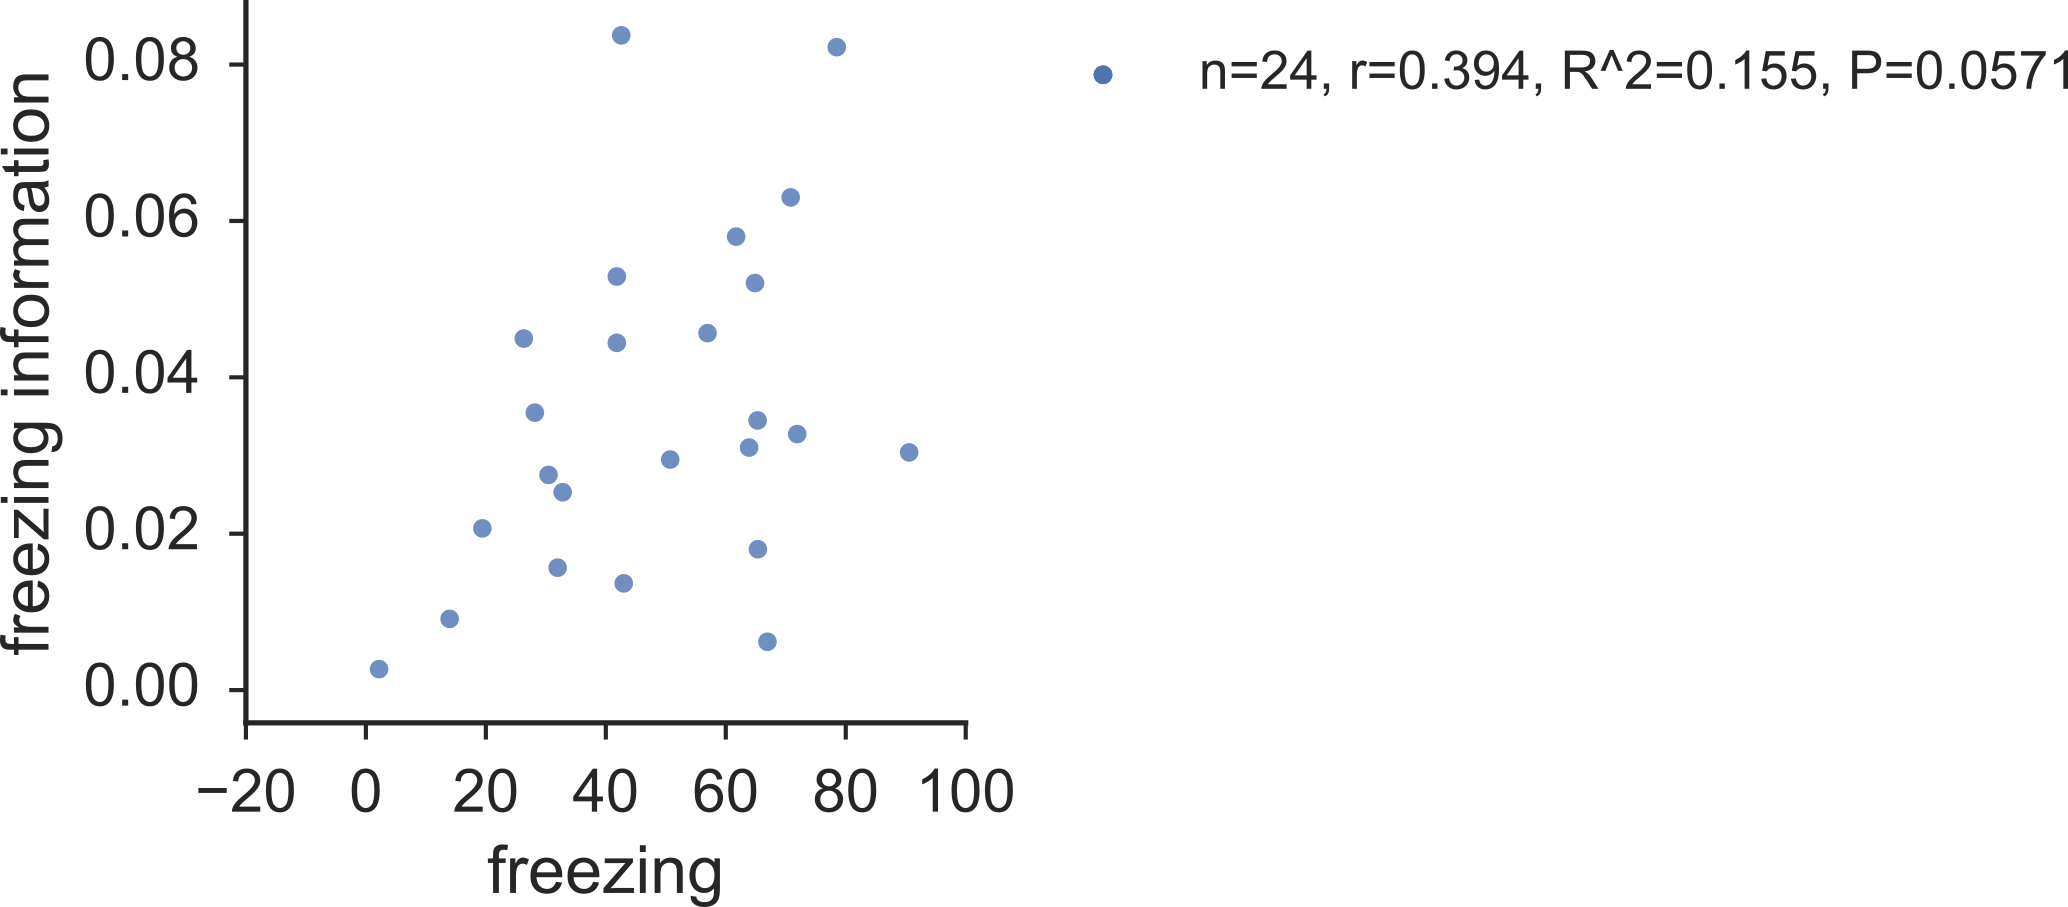
\includegraphics[width=\textwidth]{corr1.png}
        \caption{}
    \end{subfigure}
    \begin{subfigure}[t]{.5\textwidth}
        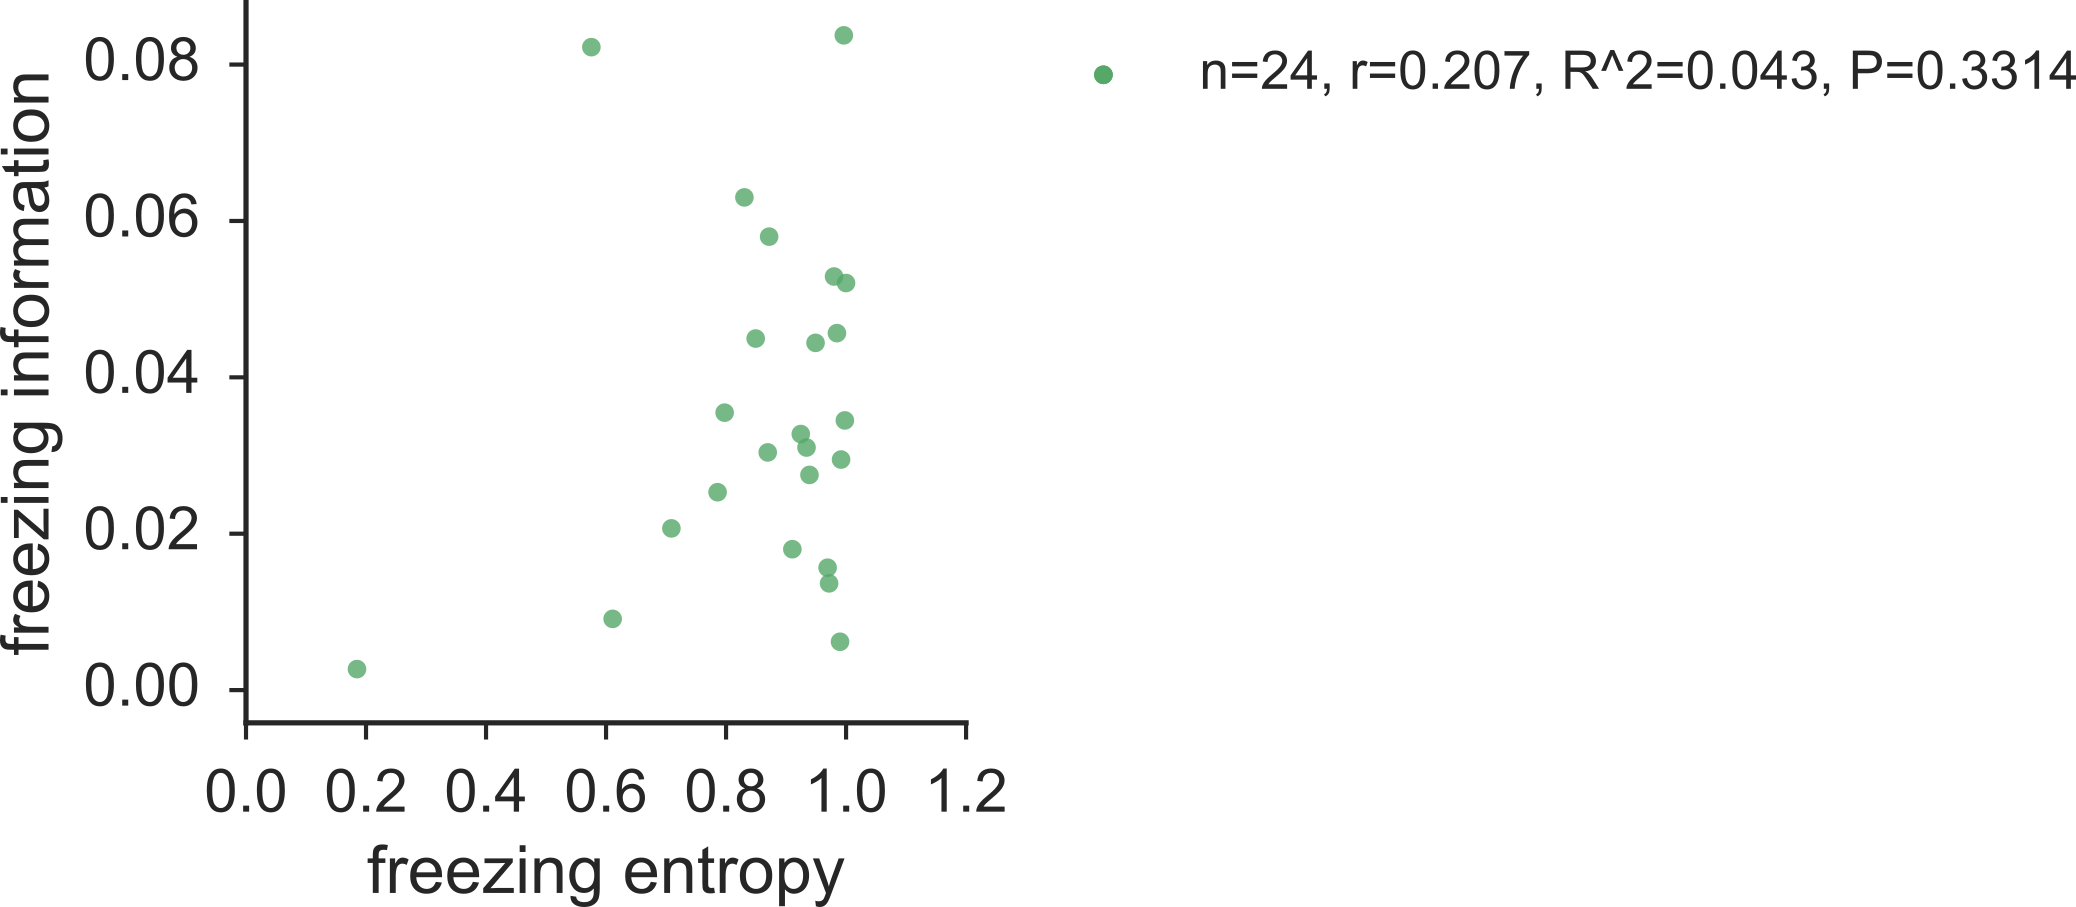
\includegraphics[width=\textwidth]{corr2.png}
        \caption{}
    \end{subfigure}
    \begin{subfigure}[t]{.5\textwidth}
        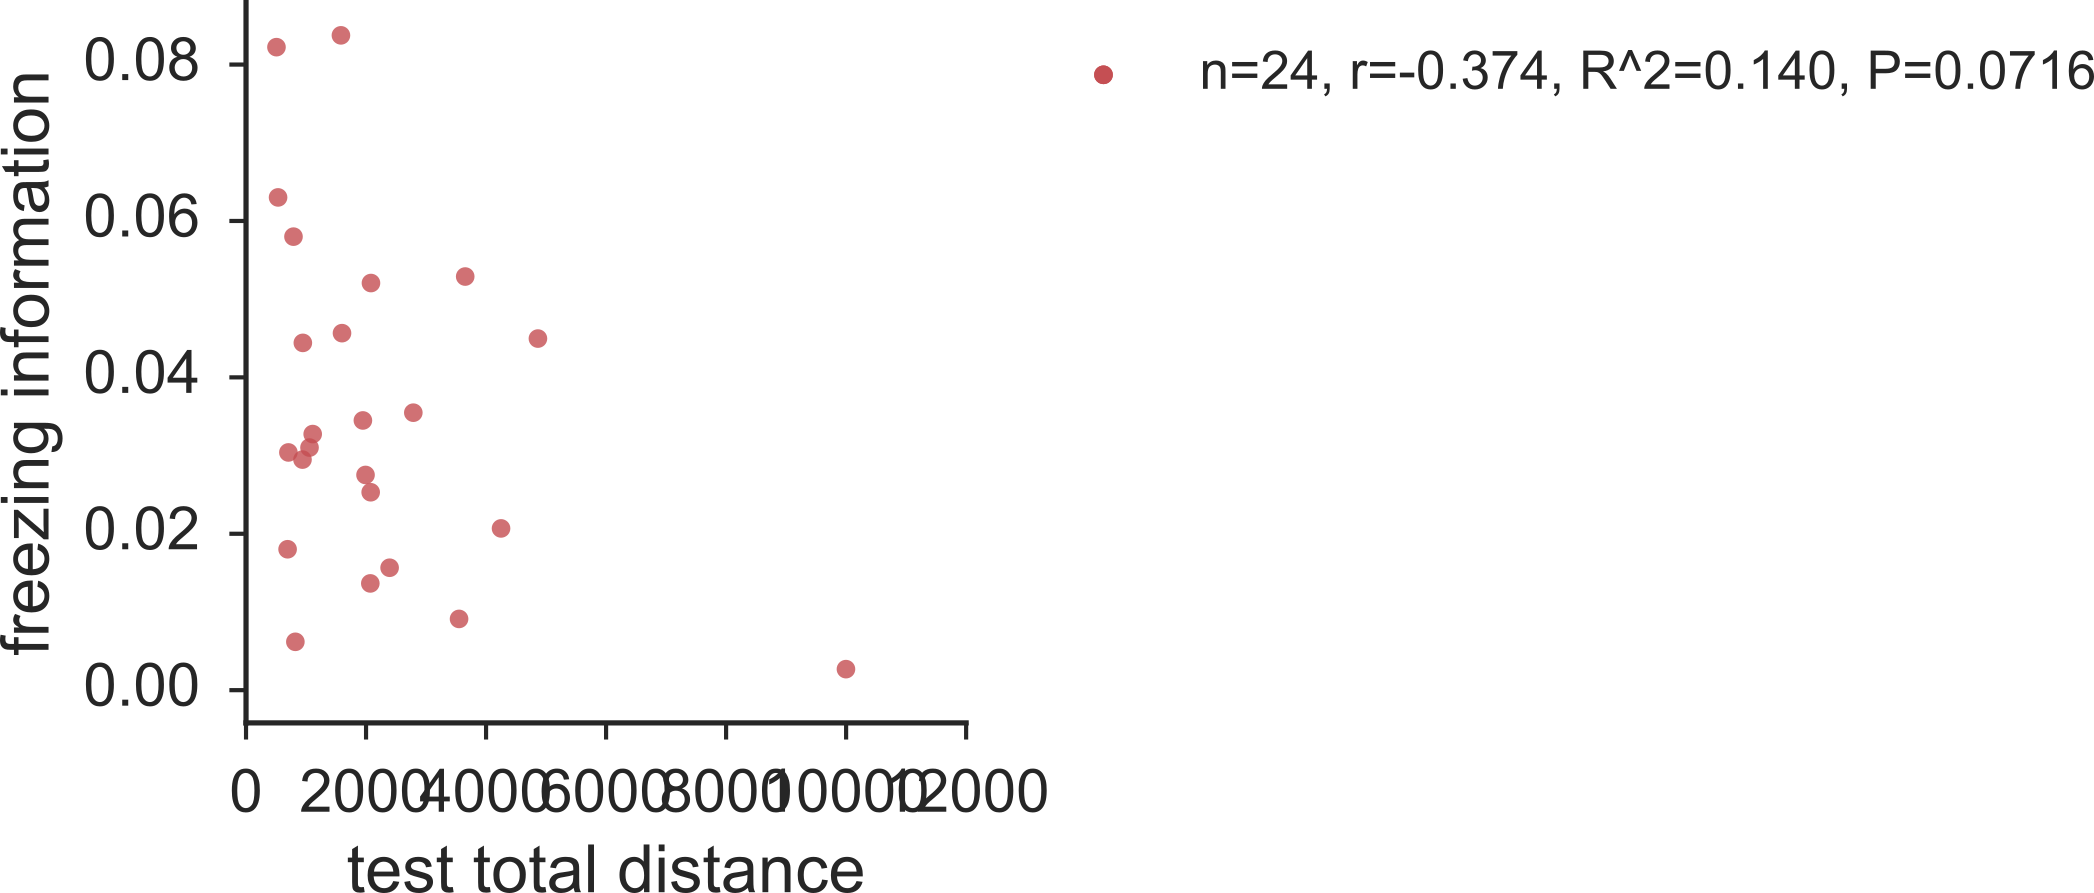
\includegraphics[width=\textwidth]{corr3.png}
        \caption{}
    \end{subfigure}
    \begin{subfigure}[t]{.5\textwidth}
        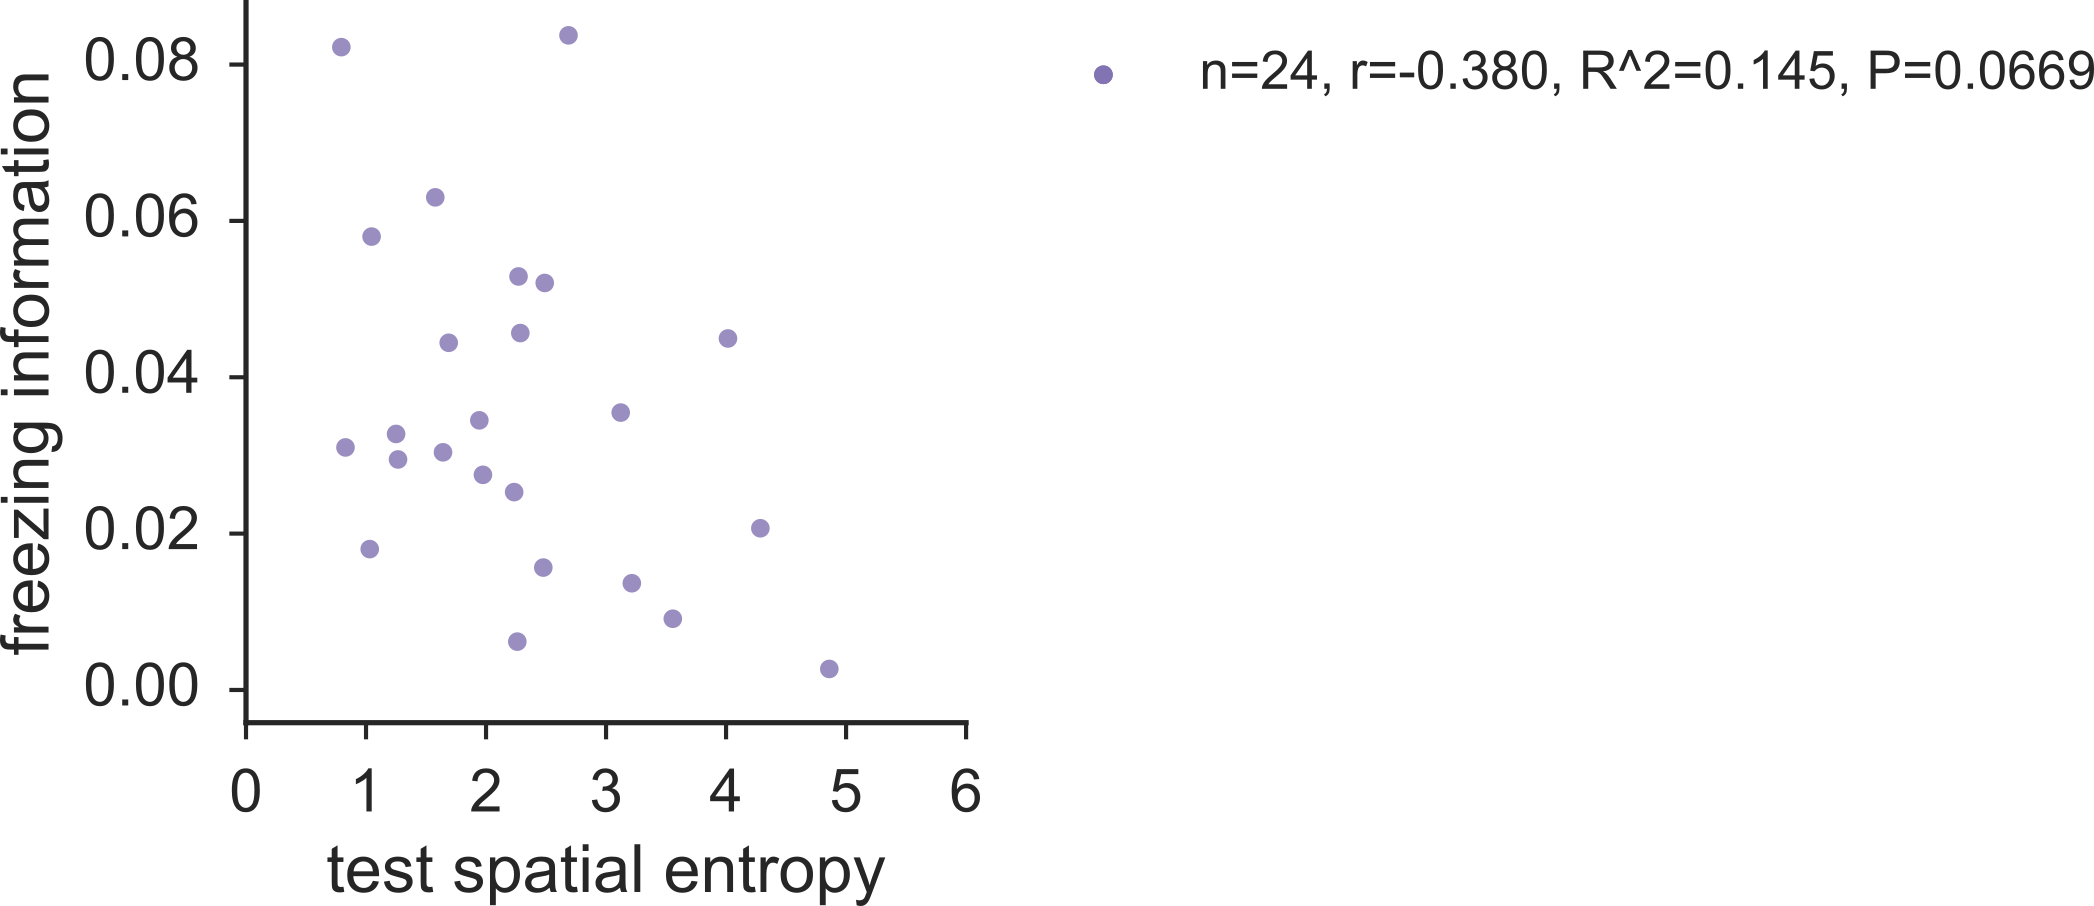
\includegraphics[width=\textwidth]{corr4.png}
        \caption{}
    \end{subfigure}
    \caption{Scatter plots of varies behaviour measurement against freezing information, in pooled \gls{wt}, \gls{wt}-\glu and \gls{tg}-\glu. Given there is no group difference between the three groups, if any of the behaviour factor is confounding, the it will contribute to within-group difference and correlate with freezing information. We have found no significant correlations. However the near significance of percent freezing and spatial entropy correlations will need further investigation. \label{f.ad.corrs}}
\end{figure}

\pagebreak 




\begin{figure}[h]
    \begin{subfigure}[h]{\textwidth}
        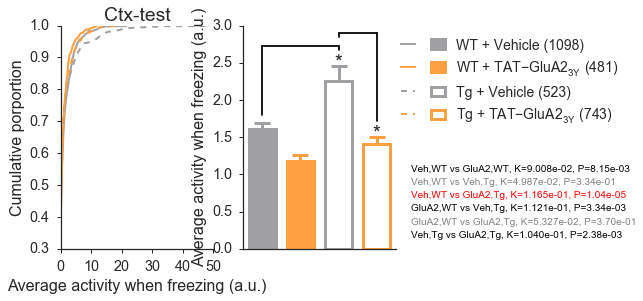
\includegraphics[width=\textwidth]{activity_freezing.png}
        \caption{\label{f.ad.actf}}
    \end{subfigure}
    \begin{subfigure}[h]{\textwidth}
        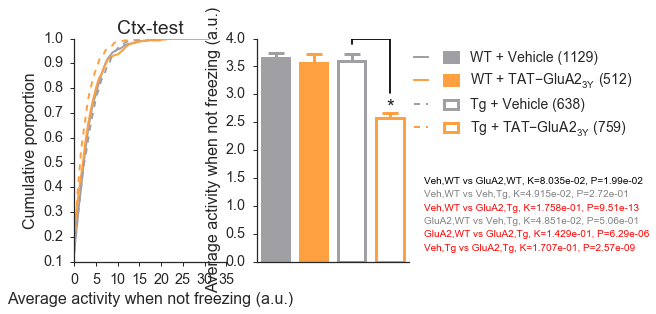
\includegraphics[width=\textwidth]{activity_moving.png}
        \caption{\label{f.ad.actnf}}
    \end{subfigure}
    \caption{Average cell activity during \subref{f.ad.actf} freezing and \subref{f.ad.actnf} not freezing. Cells in \gls{tg} animals have significantly higher activity during freezing, suggesting a sub-optimal encoding of freezing. Interestingly, \tglu also showed a decreased activity when the animal is not freezing, suggesting that the effect of \tglu maybe a global decrease of cell activity. \label{f.ad.activity_freezing}}
\end{figure}



\section{Discussion}
